\chapter{Conclusion}
\label{chapter:conclusion}
As a summary this dissertation, I focus on understanding the transport property of the heavy flavor in the strongly coupled quark-gluon plasma applying model-to-data comparison methodology, aiming for model improvements and uncertainty quantification.

A prerequisite for the study in an ``accurate'' modeling of the physical ingredients to be tested.
It is not so trivial to model the heavy quark transport that is coupled to an event-by-event fluctuating and evolving medium.
On the one hand, this is because the finite medium-induced radiation formation time at high energy is much greater than the mean-free-path in semi-classical transport equations, and can be comparable to the medium evolution time scales.
On the other hand, there are two compelling pictures regarding the heavy-quark-to-medium coupling: weakly coupled picture modeled by scatterings, and strongly coupled picture whose dynamics is often modeled by diffusion equations.
We developed a transport model for hard parton propagation in near equilibrium plasma. 
An improved treatment of LPM is implemented and it is shown to reduces to theoretical calculations in idealized infinite static medium limit, and captures qualitative features in a finite and evolving medium.
The model also treats the large and small momentum transfer processes with different strategies of few-body scattering and diffusion (plus diffusion-induced radiation) method, which grants flexible parametrization of diffusion-like deviations from leading order weakly coupled approach.

The transport in hot QGP stage fits into a more general ``transport'' picture including the initial production and high-virtuality evolution, hadronization near the transition temperature and decay and hadronic dynamics.
We identity a matching problem between the high-virtuality evolution and medium-induced evolution.
Currently, a unified formulation that smoothly connecting the virtuality shower and the in-medium shower is still missing, and we use a separation of phase-space to terminate vacuum showers at a scale ($Q^2$) where it is likely to receive similar amount of medium modifications to the transverse momentum ($\Delta k_\perp^2 \sim Q^2$).
The exact location of the separation scale is then treated as an uncertainty of the model.

Finally, we apply the Bayesian analysis to infer the model parameter distribution by comparing to heavy flavor measurements at both RHIC and the LHC.
The model parameters includes uncertainties such as in-medium coupling strength, energy loss starting time, match scale between vacuum and medium-induced shower, diffusion versus scattering model, as well as parametrized deviations from weakly coupled calculations.
The calibrated parameters is able to describe the experimental obserables within 30\% uncertainty.
This level of agreement is still not enough to make the best use of future high-precision measurements, and we shall listed a few possible improvements for future studies in the end.

\begin{figure}
\centering
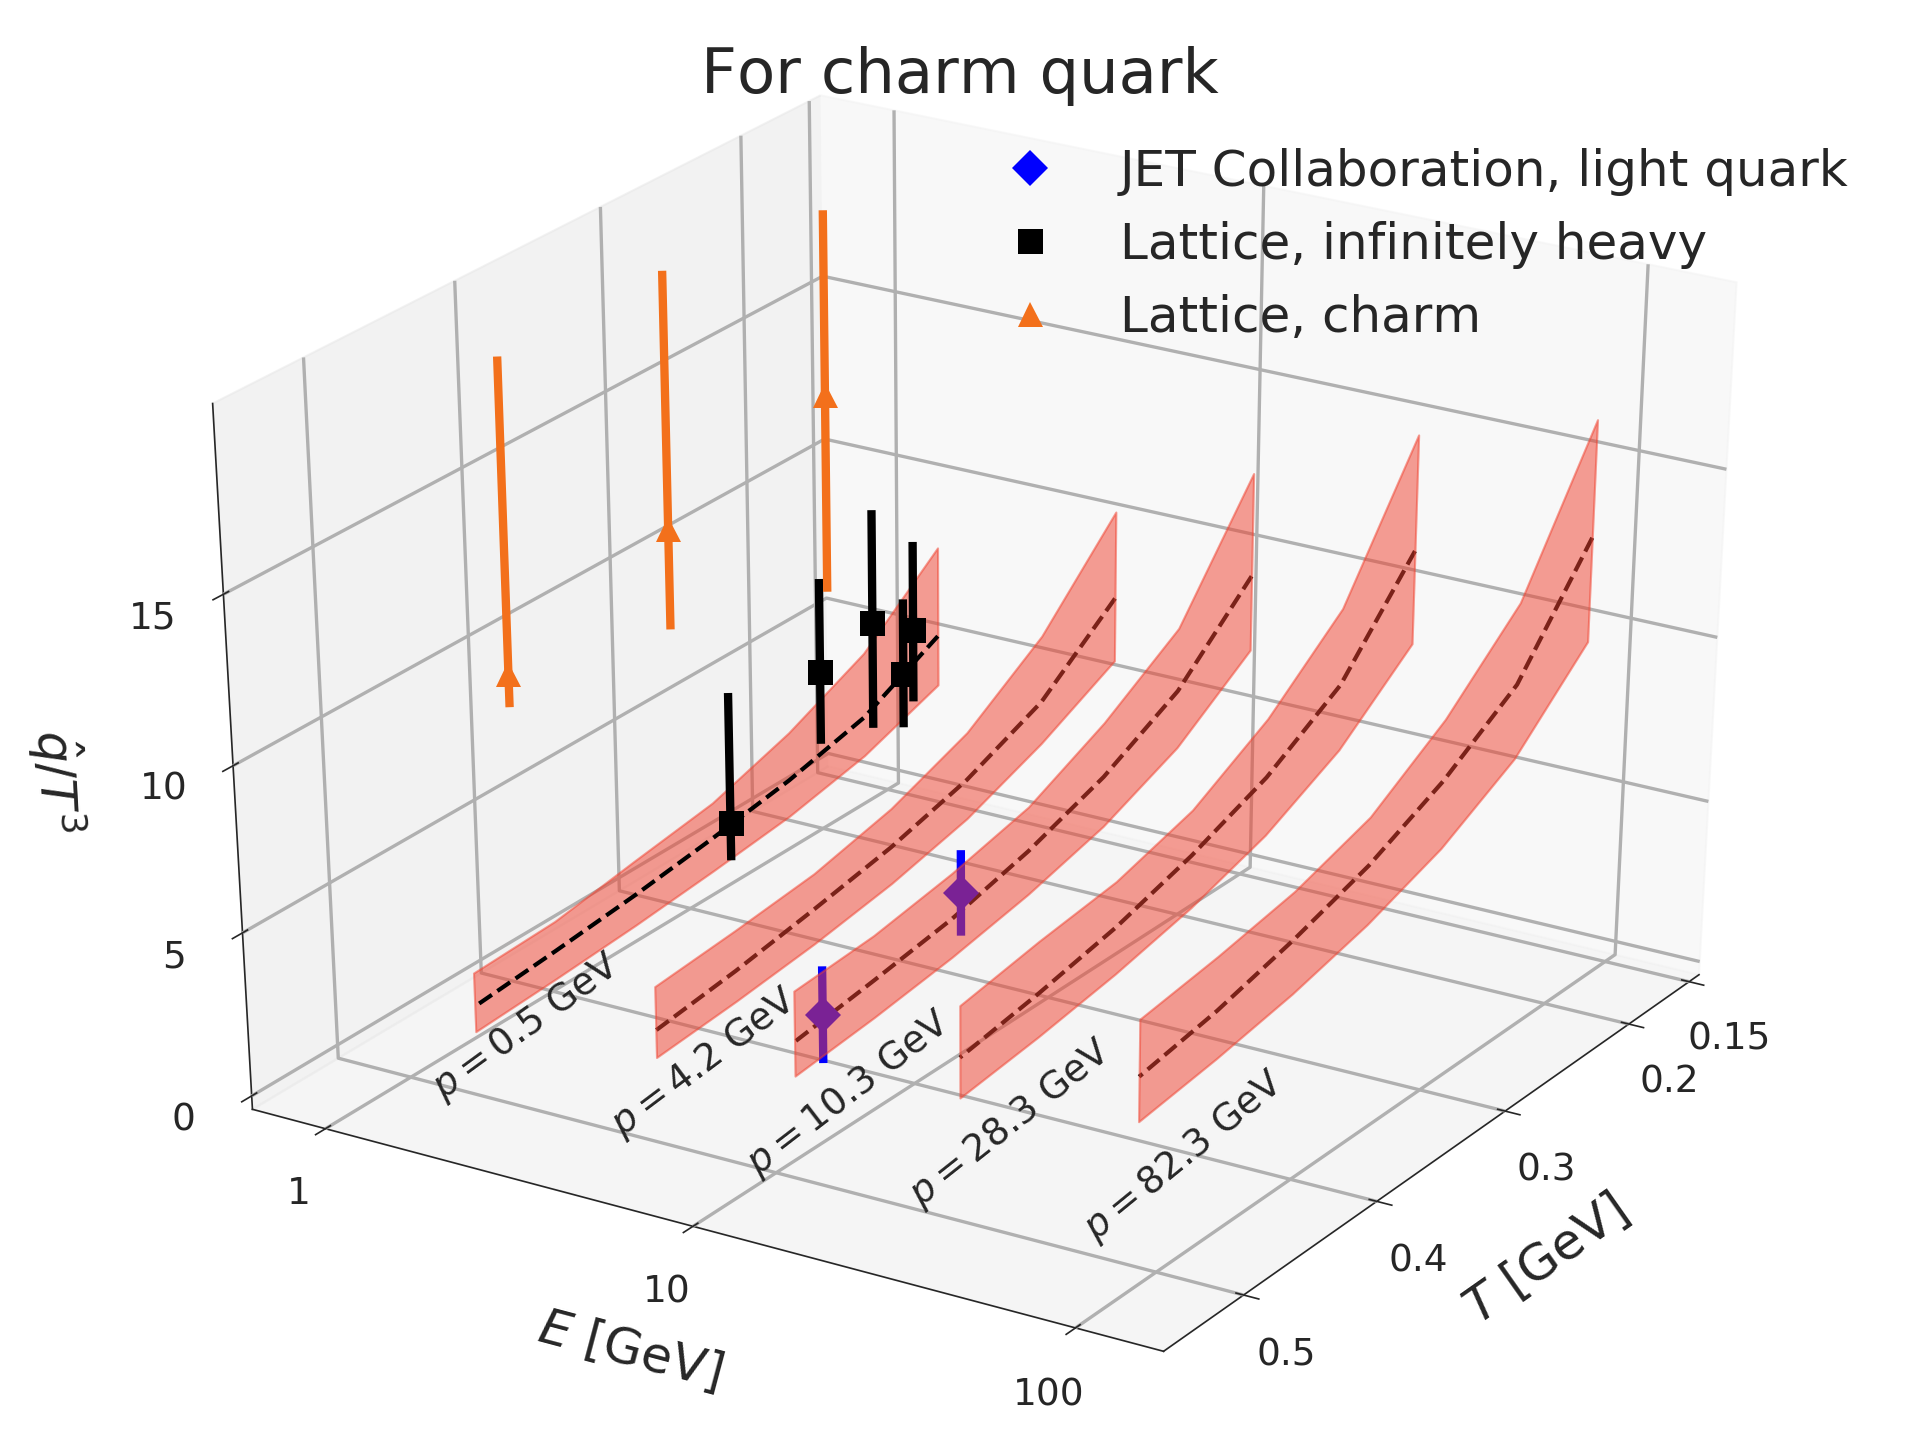
\includegraphics[width=.7\textwidth]{qhat_posterior_3D.png}
\caption{}
\label{fig:conlusion}
\end{figure}

We highlight the progress of this work in the conclusion figure \ref{fig:conlusion}.
It visualizes $90\%$ credible region of the energy and momentum dependence of the heavy quark momentum diffusion transport parameter $\hat{q}$ scaled by $T^3$.
We found $\hat{q}/T^3$ gradually increases with $\ln E$ and displays an enhancement near the critical temperature.
Studying heavy flavor helps to connect the knowledge of in-medium transport properties at very high momentum (light limit) and very low momentum (static sources limit).
At relatively high momentum $p\sim 10$ GeV, it is consistent to the light quark transport parameter extracted by the JET Collaboration (blue).
At low momentum $p\sim 0.5$ GeV, it is consistent with lattice calculations in the heavy quark limit (black).
Future study with improved flavor dependence may be needed to understand the impact of using the ``heavy' limit in dynamical model.
In the current present calibration, the effective in-medium strong coupling constant is about $0.3$, and only contribute a small fraction of the extracted $\hat{q}$ parameter.
The rest comes from the parametric contribution whose origin can be either perturbative or non-perturbative; either way, it suggests the necessity to model beyond leading order physics.

Considering the advent of future high-precision hard probe measurements in heavy-ion collisions,
we summarize a few points of improvements that may help to reduce or estimate the theoretical and modeling uncertainty of hard probes application.
\begin{itemize}
\item An interpolation formula between vacuum and medium-induced radiation
\item Correlation among multiple emissions in the presence of medium.
\item Off equilibrium correction to the linearized transport equation.
\item A calibration with simultaneous tuning bulk and hard sector.
\item The use of less Glauber-model-dependent observables.
\item Dynamical hadronization model and improved treatment of energy loss in the hadronic stage.
\end{itemize}